\section{Variation of  ``Quark-Gluon'' Sample Selection Criteria }
%\label{sec:globalFitStability} % uncomment if label used. 

A variation on the quark-gluon selection criteria has been studied by varying the 
estimation of the \ntrk\ that corresponds to a given efficiency for truth quark and gluon jets as described below.

The constants $m$ and $c$ are found by finding the value of \ntrk\ 
that corresponds to a given efficiency for truth quark and gluon jets in 
\pT\ bins and fitting the results. For each \pT\ bin the number of tracks 
closest to the chosen selection efficiency is found. Since this is an integer 
number of tracks and does and does not correspond exactly to the selection efficiency 
a correction is applied by estimating the fractional number of tracks that corresponds 
to the selection  efficiency  by carrying out a linear interpolation between the efficiencies 
for the selected bin and its nearest neighbour. The uncertainty on this value is then estimated using 
binomial uncertainties. 



The jet \pT\ bin edges are chosen to be 
480, 500, 520, 540, 560, 580, 600, 625, 650, 700, 750, 800, 900, 1000, 1400, 
1600, 1800, 2000, 2500, 3000, 3500, 4000, 5000, 6000\,\GeV. An example of the \ntrk cumulative 
distribution for truth quark and gluon jets satisfying $800 < \pT < 900\,\GeV$ is shown in
Fig.~\ref{fig:ntrk_cumulative_app}.


\begin{figure}[htb]
 \centering
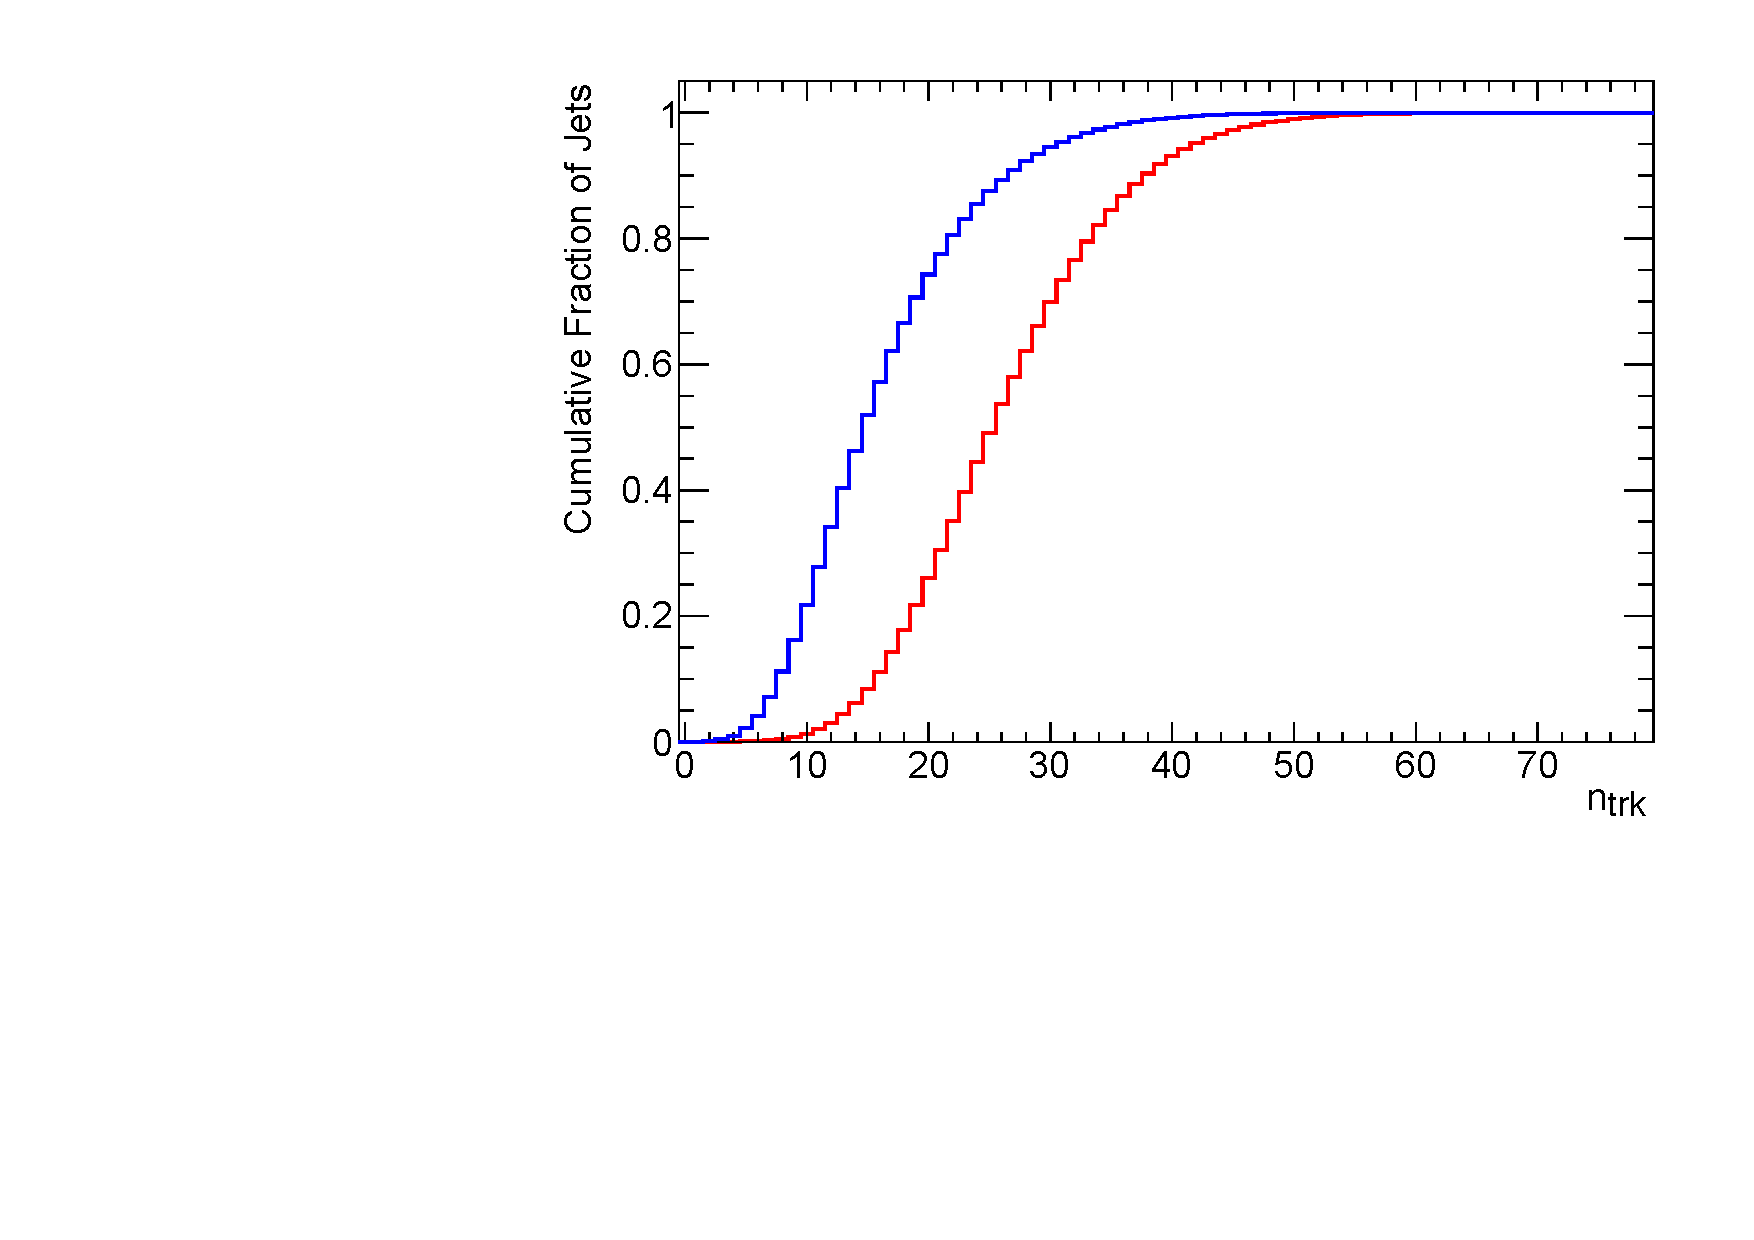
\includegraphics[width=0.75\textwidth]{figures/tagging_variation/Cumulative_ntrk_distribution_12_800_900GeV.pdf}
\caption{The cumulative distribution of \ntrk\ for truth quark (blue) and gluon (red) initiated jets 
satisfying $800 < \pT < 900\,\GeV$.  \label{fig:ntrk_cumulative_app}}
\end{figure}


The constants for Eq.~\ref{eq:nqg2} are found for quark and gluon selection efficiencies from 
65\% to 95\% in 5\% steps. The plot of the value of \ntrk\ that satisfies the selection efficiencies 
of 70, 75 and 80\% are shown in Fig.~\ref{fig:qg_selection_curves_app} along with the best fit using Eq.~\ref{eq:nqg2}.
The values of the constants for both quark and gluon selections are summarised in 
Tables~\ref{table:truthQuarkSelectionEfficiencies_app} and \ref{table:truthGluonSelectionEfficiencies_app}. 
The fit for a selection efficiency of 75\% has a $\chi^2$ of $33.5$ (quark-selection) and $2.6$ 
(gluon-selection) for 21 degrees of freedom. 

The value of \ntrk\ that satisfies the selection efficiency plateaus above 4000\,\GeV\ indicating a possible saturation effect. As a cross check the data is fitted to an alternative fit function 
\begin{equation}
n_{\mathrm{q(g)}} = {c + m \ln(\pT) + n \sqrt{\ln(\pT)}}. \label{eq:nqg3}
\end{equation}
This improves the $\chi^2$ of the fit for a selection efficiency of 75\% for quark-selection from
$33.5$ to $25.1$ and for gluon-selection from $2.6$ to $1.6$.  The improved fit is shown in Fig.~\ref{fig:qg_selection_curves2} and the values of the constants for both quark and gluon selections 
are summarised in 
Tables~\ref{table:truthQuarkSelectionEfficiencies2} and \ref{table:truthGluonSelectionEfficiencies2}. 

\clearpage


\begin{table}[h]
	\centering 
		\caption{ Values of constants $m$ and $c$ from Eq.~\ref{eq:nqg2} such that $ \ntrk  \le \nq $ 
		for truth quark jets for a range of efficiencies  from 65 to 95\%. 
		\label{table:truthQuarkSelectionEfficiencies_app}
		}
	\begin{tabular}{SSSS}
	\toprule
\multicolumn{1}{c}{Truth-$q$ selection efficiency}   & \multicolumn{1}{c}{Truth-$g$ selection efficiency} &  \multicolumn{1}{c}{$c$}  &  \multicolumn{1}{c}{$m$} \\
\midrule 
0.95 & 0.732 & -27.568 & 8.789 \\
0.90 & 0.563 & -21.518 & 7.269 \\
0.85 & 0.447 & -17.646 & 6.304 \\
0.80 & 0.350 & -14.956 & 5.610 \\
0.75 & 0.278 & -12.600 & 5.022 \\
0.70 & 0.221 & -10.691 & 4.536 \\
0.65 & 0.174 & -8.990 & 4.105 \\
\bottomrule
\end{tabular}
\end{table}

\begin{table}[h]
	\centering 
		\caption{ Values of constants $m$ and $c$ from Eq.~\ref{eq:nqg2} such that $ \ntrk  \ge \ngluon $ 
		for truth quark jets for a range of efficiencies  from 65 to 95\%. 
		\label{table:truthGluonSelectionEfficiencies_app}
		}
	\begin{tabular}{SSSS}
	\toprule
\multicolumn{1}{c}{Truth-$g$ selection efficiency}   & \multicolumn{1}{c}{Truth-$q$ selection efficiency} &  \multicolumn{1}{c}{$c$}  &  \multicolumn{1}{c}{$m$} \\
\midrule 
 0.95 & 0.586 & -7.541 & 3.233 \\
0.90 & 0.456 & -8.980 & 3.779 \\
0.85 & 0.377 & -10.419 & 4.230 \\
0.80 & 0.320 & -11.964 & 4.659 \\
0.75 & 0.274 & -13.376 & 5.047 \\
0.70 & 0.234 & -14.937 & 5.446 \\
0.65 & 0.202 & -16.466 & 5.834 \\
\bottomrule
\end{tabular}
\end{table}


\begin{table}[h]
	\centering 
		\caption{ Values of constants $m$ and $c$ from Eq.~\ref{eq:nqg3} such that $ \ntrk  \le \nq $ 
		for truth quark jets for a range of efficiencies  from 70 to 80\%. 
		\label{table:truthQuarkSelectionEfficiencies2}
		}
	\begin{tabular}{SSSSS}
	\toprule
\multicolumn{1}{c}{Truth-$q$ selection efficiency}   & \multicolumn{1}{c}{Truth-$g$ selection efficiency} &  \multicolumn{1}{c}{$c$}  &  \multicolumn{1}{c}{$m$} &  \multicolumn{1}{c}{$n$} \\
\midrule 
0.80 & 0.350 & -139.822 & -11.714 & 93.100 \\
0.75 & 0.278 & -128.174 & -11.001 & 86.141 \\
0.70 & 0.221 & -128.255 & -11.755 & 87.604 \\
\bottomrule
\end{tabular}
\end{table}


\begin{table}[h]
	\centering 
		\caption{ Values of constants $m$ and $c$ from Eq.~\ref{eq:nqg3} such that $ \ntrk  \ge \ngluon $ 
		for truth quark jets for a range of efficiencies  from 70 to 80\%. 
		\label{table:truthGluonSelectionEfficiencies2}
		}
	\begin{tabular}{SSSSS}
	\toprule
\multicolumn{1}{c}{Truth-$g$ selection efficiency}   & \multicolumn{1}{c}{Truth-$q$ selection efficiency} &  \multicolumn{1}{c}{$c$}  &  \multicolumn{1}{c}{$m$} &  \multicolumn{1}{c}{$n$}  \\
\midrule 
0.80 & 0.320 & -99.796 & -7.839 & 66.301 \\
0.75 & 0.274 & -99.949 & -7.271 & 65.347 \\
0.70 & 0.234 & -99.774 & -6.640 & 64.077 \\
\bottomrule
\end{tabular}
\end{table}




\begin{figure}[p]
 \centering
  \subfigure[] {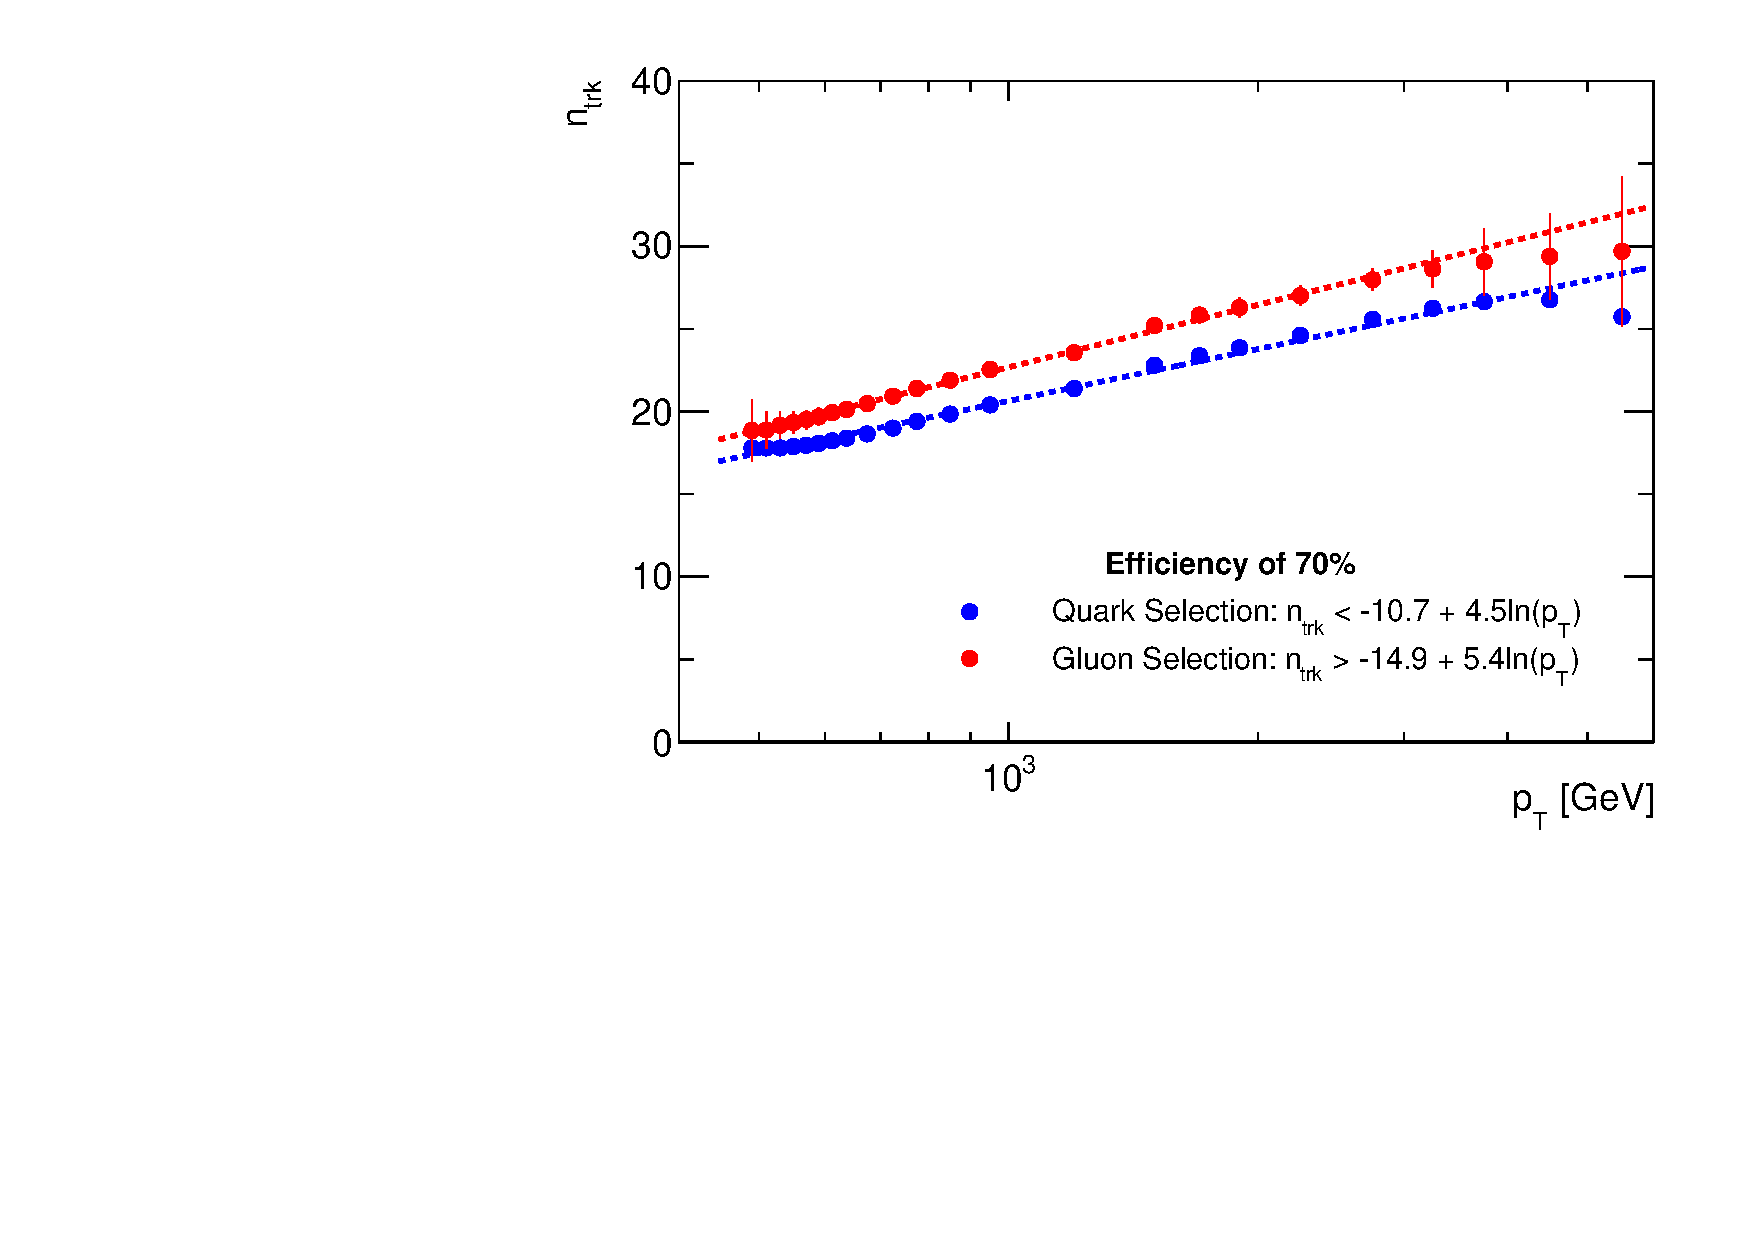
\includegraphics[width=0.60\textwidth]{figures/tagging_variation/quark_frac_selection_errors_6}}
  \subfigure[] {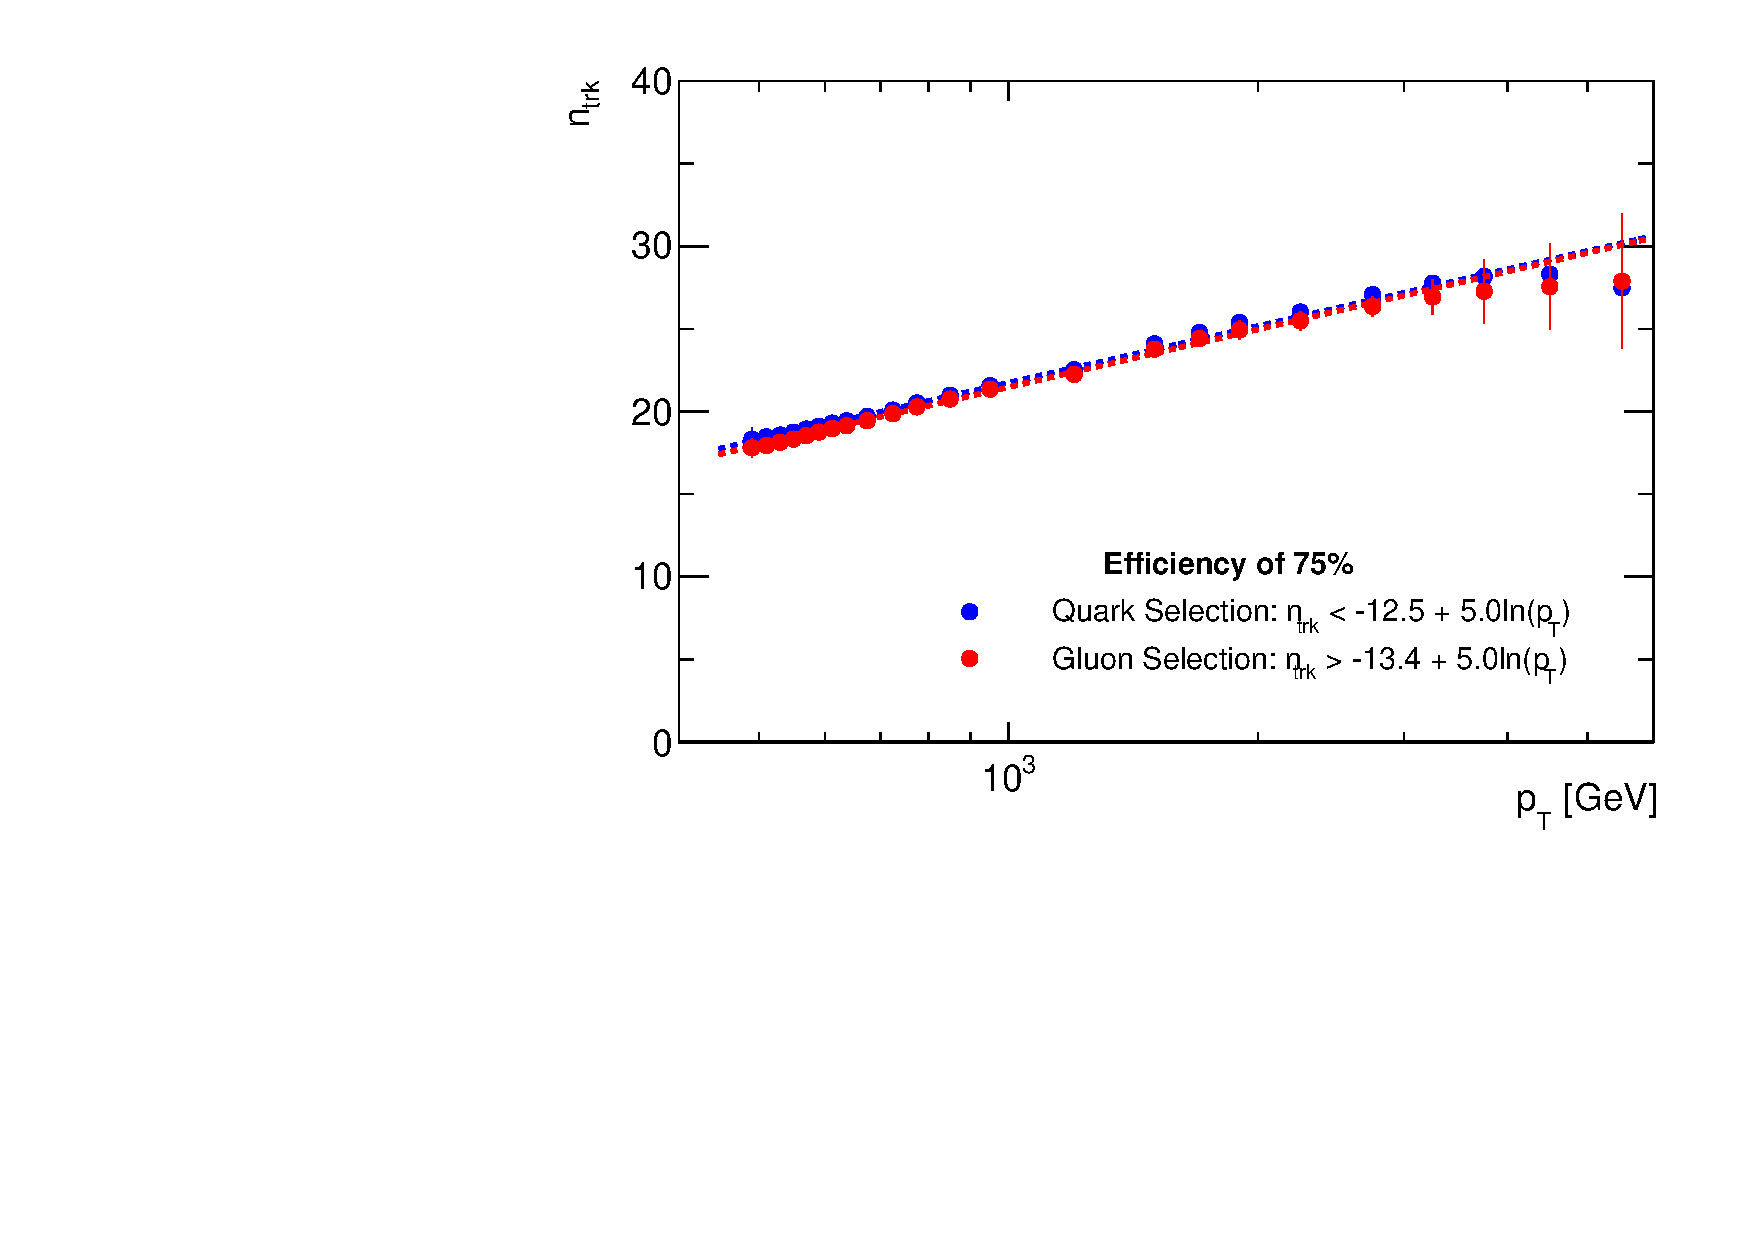
\includegraphics[width=0.60\textwidth]{figures/tagging_variation/quark_frac_selection_errors_5}}
  \subfigure[] {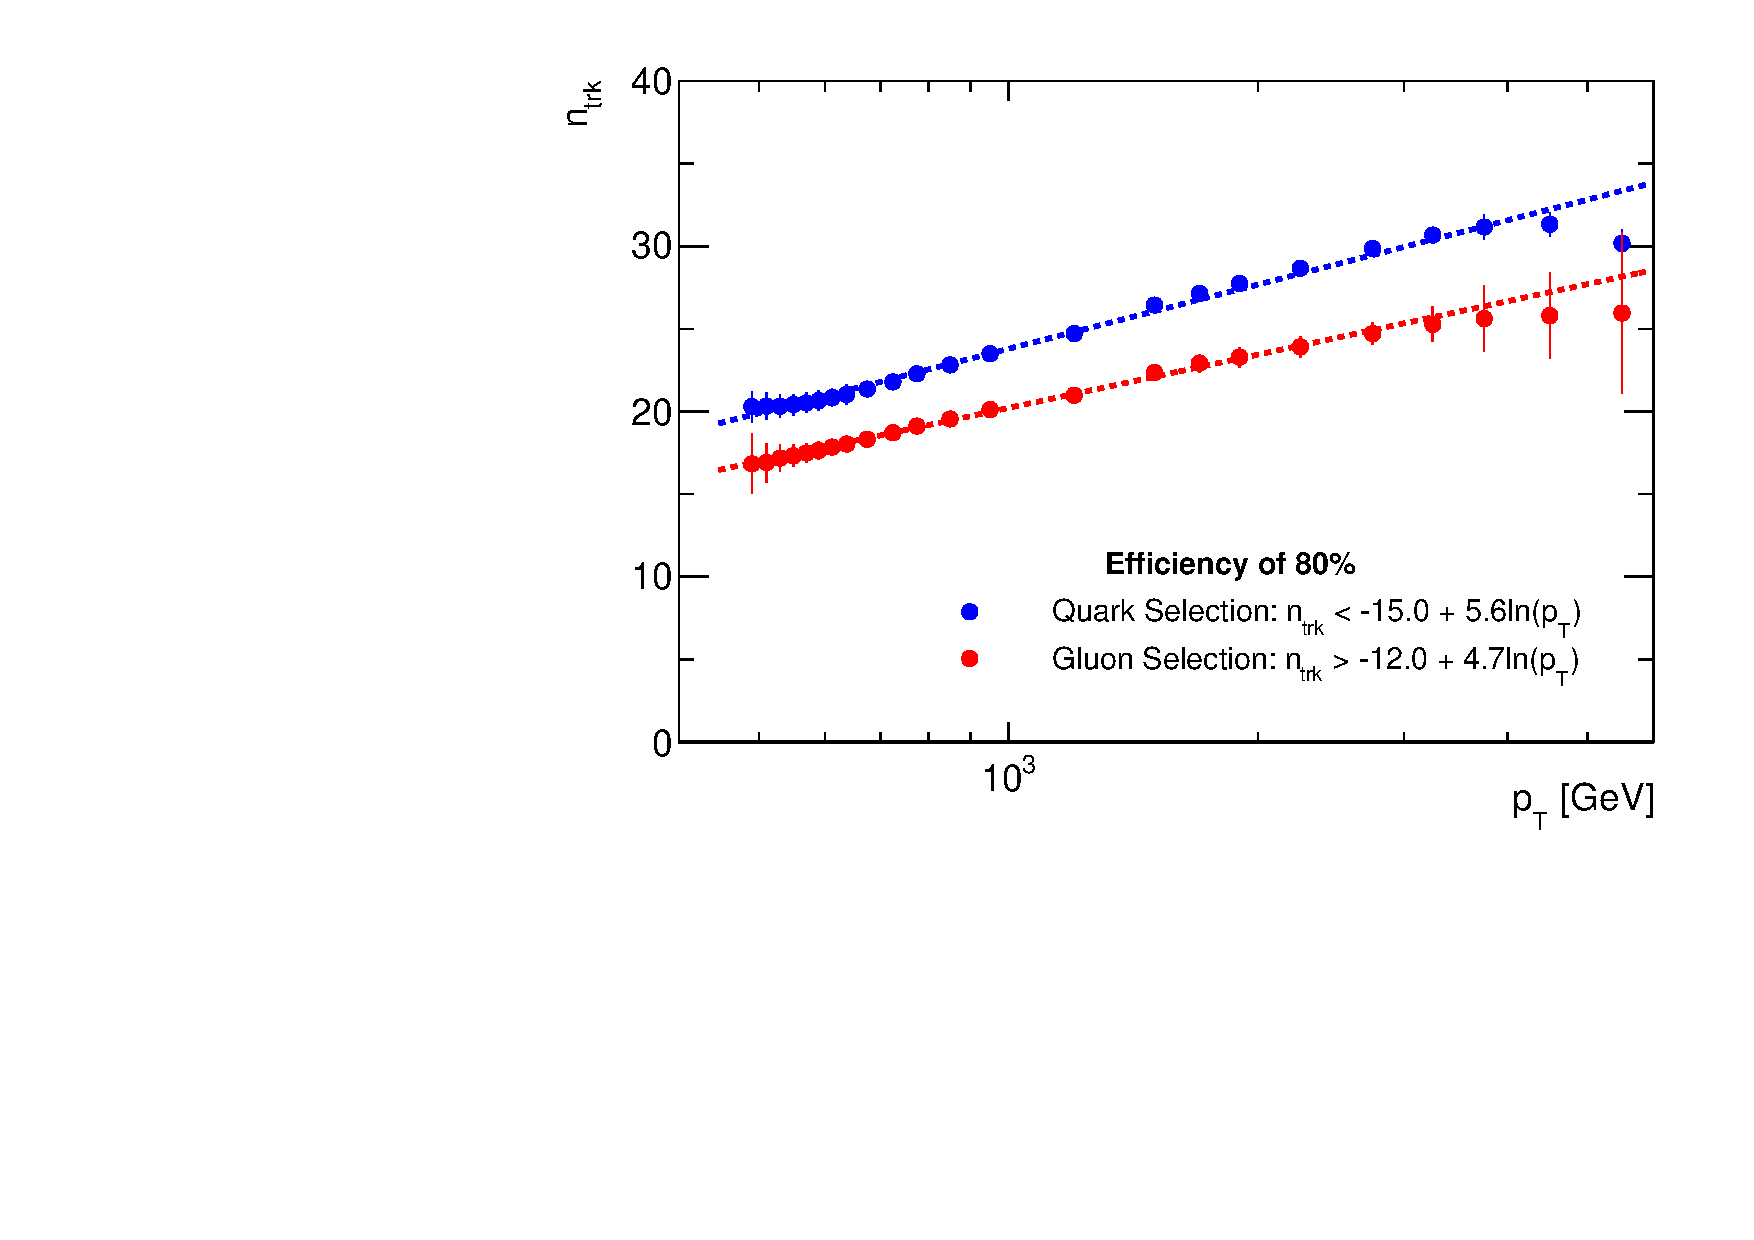
\includegraphics[width=0.60\textwidth]{figures/tagging_variation/quark_frac_selection_errors_4}}

\caption{ The values of \ntrk\ for (a) 70\%,  (b) 75\%  and (c) 80\% quark (blue) and gluon (red) 
selection efficiencies in each \pT\ bin along with the best fit to Eq.~\ref{eq:nqg2}.
 \label{fig:qg_selection_curves_app}}
\end{figure}

\begin{figure}[p]
 \centering
  \subfigure[] {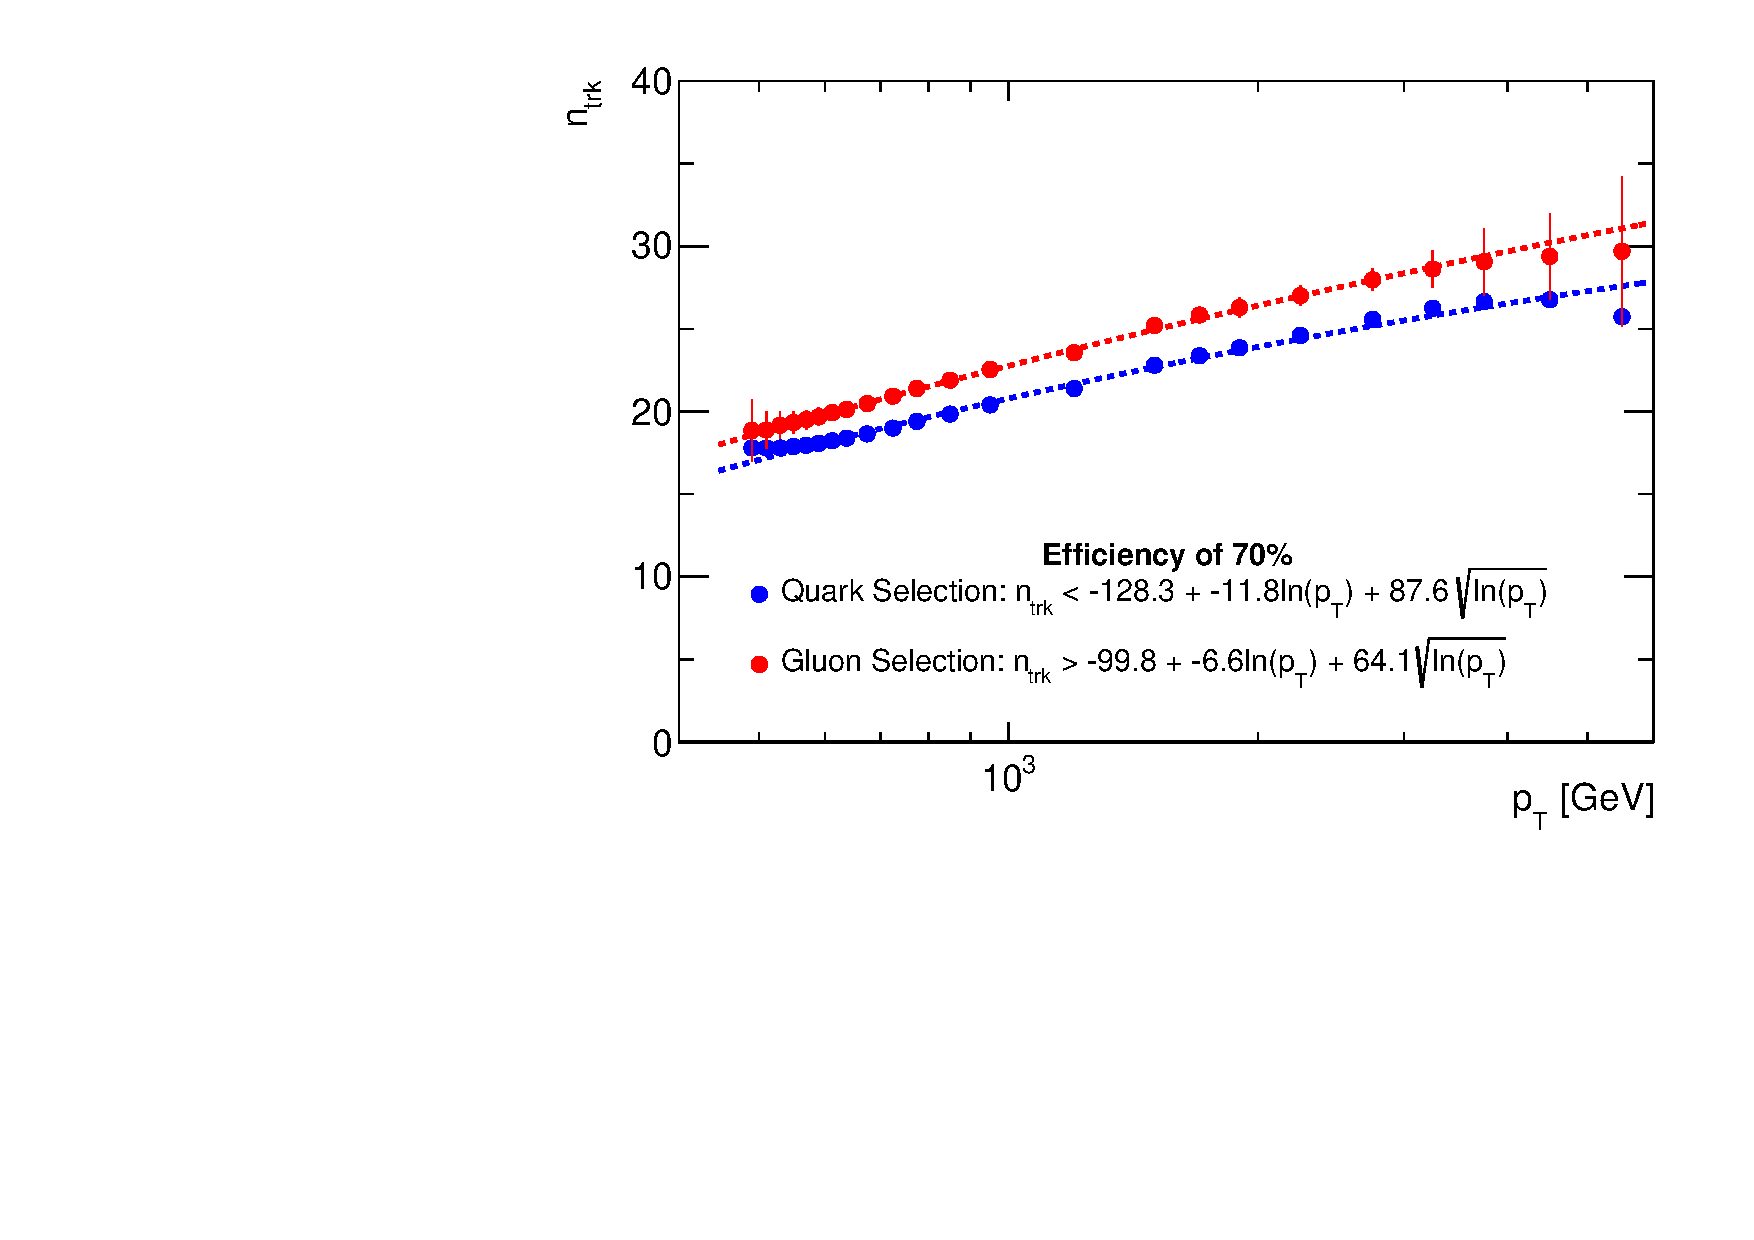
\includegraphics[width=0.60\textwidth]{figures/tagging_variation/quark_frac_newFit_selection_errors_6}}
  \subfigure[] {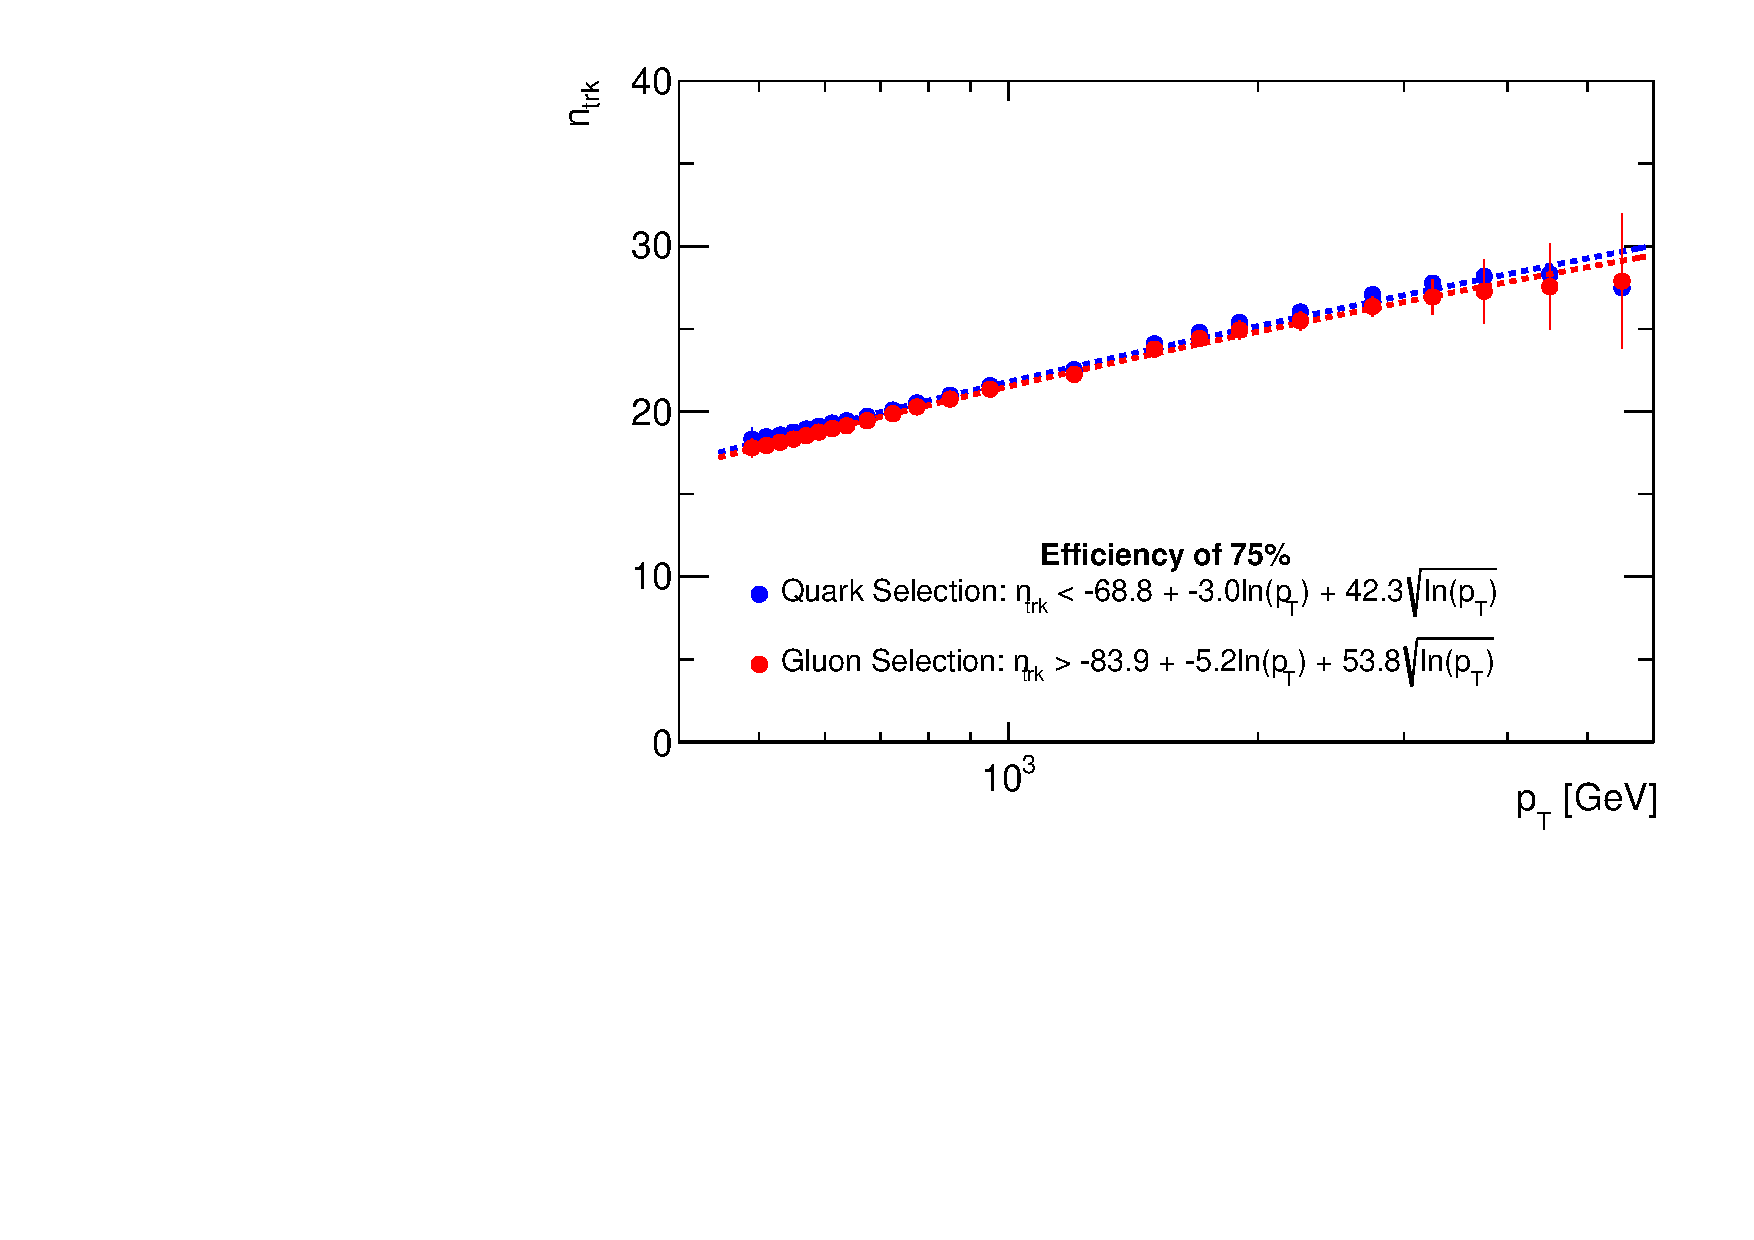
\includegraphics[width=0.60\textwidth]{figures/tagging_variation/quark_frac_newFit_selection_errors_5}}
  \subfigure[] {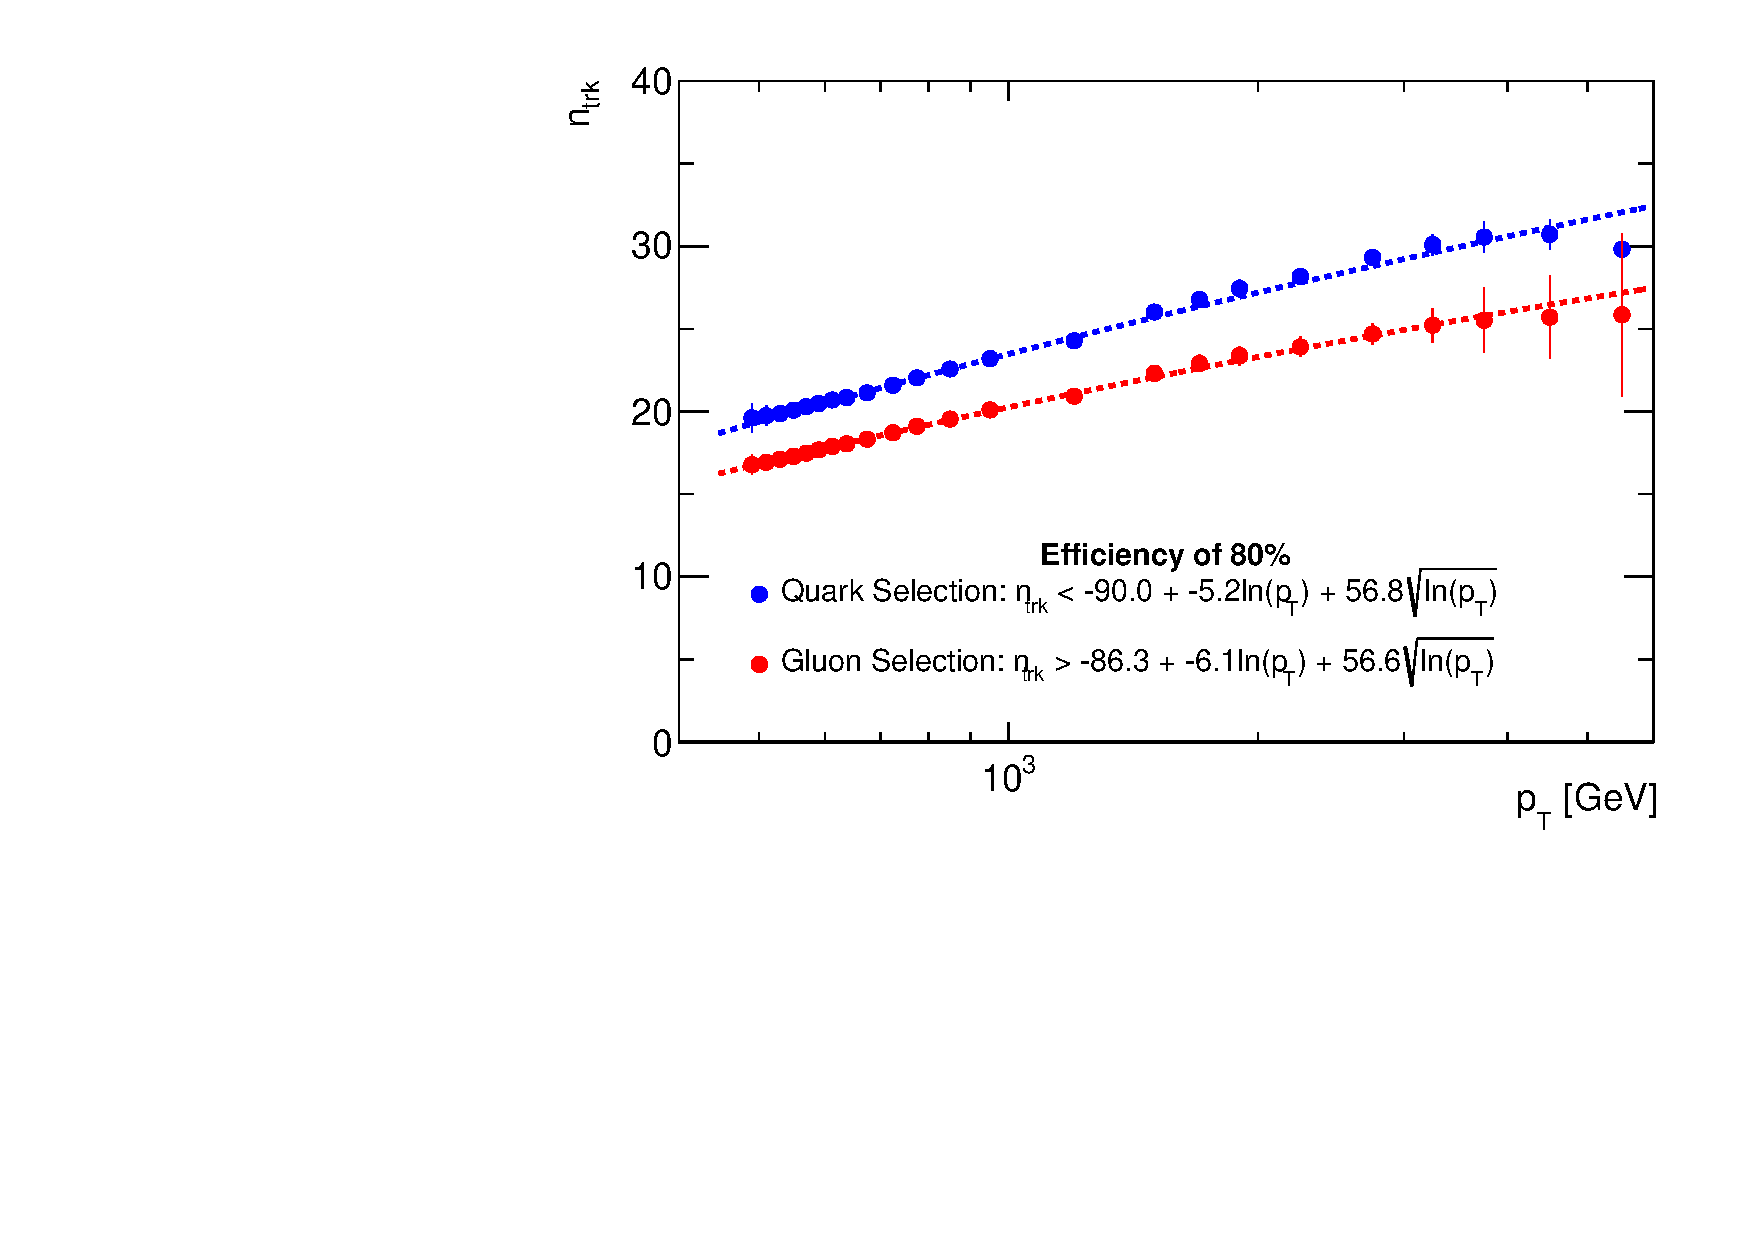
\includegraphics[width=0.60\textwidth]{figures/tagging_variation/quark_frac_newFit_selection_errors_4}}

\caption{ The values of \ntrk\ for  (a) 70\%,  (b) 75\%  and (c) 80\% quark  quark (blue) and gluon (red) 
selection efficiencies in each \pT\ bin along with the best fit to Eq.~\ref{eq:nqg3}.
 \label{fig:qg_selection_curves2}}
\end{figure}


\subsubsection{Signal Selection Efficiencies}


The selection criteria for a single jet gluon selection efficiency of 75\% is applied to the \Hprime\ 
sample described in in section~\ref{sec:hprime} are given in Table~\ref{table:HprimeselctionEfficiency_app}. 
If the selection works perfectly the expected selection efficiency for the \Hprime\ sample would be 56.3\% ($0.75^2$). 
The actual selection efficiencies range between 51.9\% for a 2\,\TeV\ signal to 57.4\% for a 7\,\TeV\ signal. 

The actual fraction of \Hprime\ events that decay to two gluons is less than 100\% due to gluon splitting and other showering 
effects and ranges from 91.3 to 95.4\%. The variation between the expected efficiency (56.3\% of the truth efficiency) 
is plotted in Fig.~\ref{fig:HPrime_efficiency_difference}. The average difference for is approximately 3.3\% for both selection criteria.

There is negligible difference between the two selection criteria so the simpler choice as given in Eq.~\ref{eq:nqg2} will be used.



\begin{table}[h]
	\centering 
		\caption{ The signal selection efficiency for a fully simulated \Hprime\ decaying to two gluons with requiring two jets to 
		pass the 75\% single jet criteria given in Eq.~\ref{eq:nqg2} with constants from 
		Table~\ref{table:truthGluonSelectionEfficiencies_app} and the criteria given in Eq.~\ref{eq:nqg3} with constants from 
		Table~\ref{table:truthGluonSelectionEfficiencies2}.  
		The expected double tagged gluon efficiency is 56.3\%. 
		\label{table:HprimeselctionEfficiency_app}
		}
	\begin{tabular}{SSSS}
	\toprule
\multicolumn{1}{c}{\Hprime\ Mass (\GeV)}   & \multicolumn{3}{c}{Selection efficiency(\%)} \\
\multicolumn{1}{c}{} & \multicolumn{1}{c}{Eq.~\ref{eq:nqg2}} & \multicolumn{1}{c}{Eq.~\ref{eq:nqg3} ($\sqrt{}$ term)} 
& \multicolumn{1}{c}{Truth} \\
\midrule 
2000	&	51.9 & 51.8& 91.3 \\
2500	&	53.2 & 53.0& 91.7 \\
3000 	&	54.9 & 54.6& 92.3 \\
3500	&	55.3 & 55.1& 93.4 \\
4000	&	56.4 & 56.2& 93.4 \\
4500	&	56.7 & 56.7& 94.1 \\
5000	&	56.2 & 56.4& 94.3 \\
5500	&	57.2 & 57.5& 94.9 \\
6000	&	57.4 & 57.8& 95.1 \\
6500	&	57.4 & 58.3& 95.5 \\
7000	&	57.4 & 58.1& 95.4 \\\bottomrule
\end{tabular}
\end{table}


\begin{figure}[p]
 \centering
 {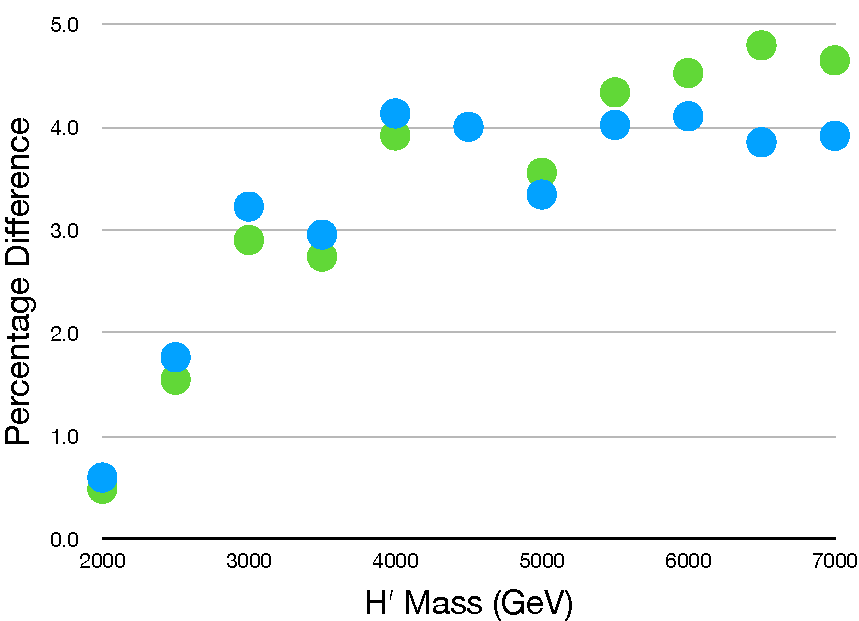
\includegraphics[width=0.60\textwidth]{figures/tagging_variation/HPrime_Efficiency_Difference}}

\caption{ The difference between the expected signal selection efficiency of 56.3\%
for a single jet selection efficiency of 75\% for \Hprime\ using  Eq.~\ref{eq:nqg2} (Blue) and
Eq.~\ref{eq:nqg3} (Green)
 \label{fig:HPrime_efficiency_difference}}
\end{figure}


